\chapter{Results}
\label{cha:results}

% This chapter presents the results. Note that the results are presented
% factually, striving for objectivity as far as possible.  The results
% shall not be analyzed, discussed or evaluated.  This is left for the
% discussion chapter.

% In case the method chapter has been divided into subheadings such as
% pre-study, implementation and evaluation, the result chapter should
% have the same sub-headings. This gives a clear structure and makes the
% chapter easier to write.

% In case results are presented from a process (e.g. an implementation
% process), the main decisions made during the process must be clearly
% presented and justified. Normally, alternative attempts, etc, have
% already been described in the theory chapter, making it possible to
% refer to it as part of the justification.

\section{Web browser}

The resulting web browser is implemented in two ways. The first as a so called screen space browser. This is a browser window within the Openspace window that can be moved around and placed on the screen where the user wants it. See figure \ref{fig:screenspace}.

\begin{figure}[!h]
\centering
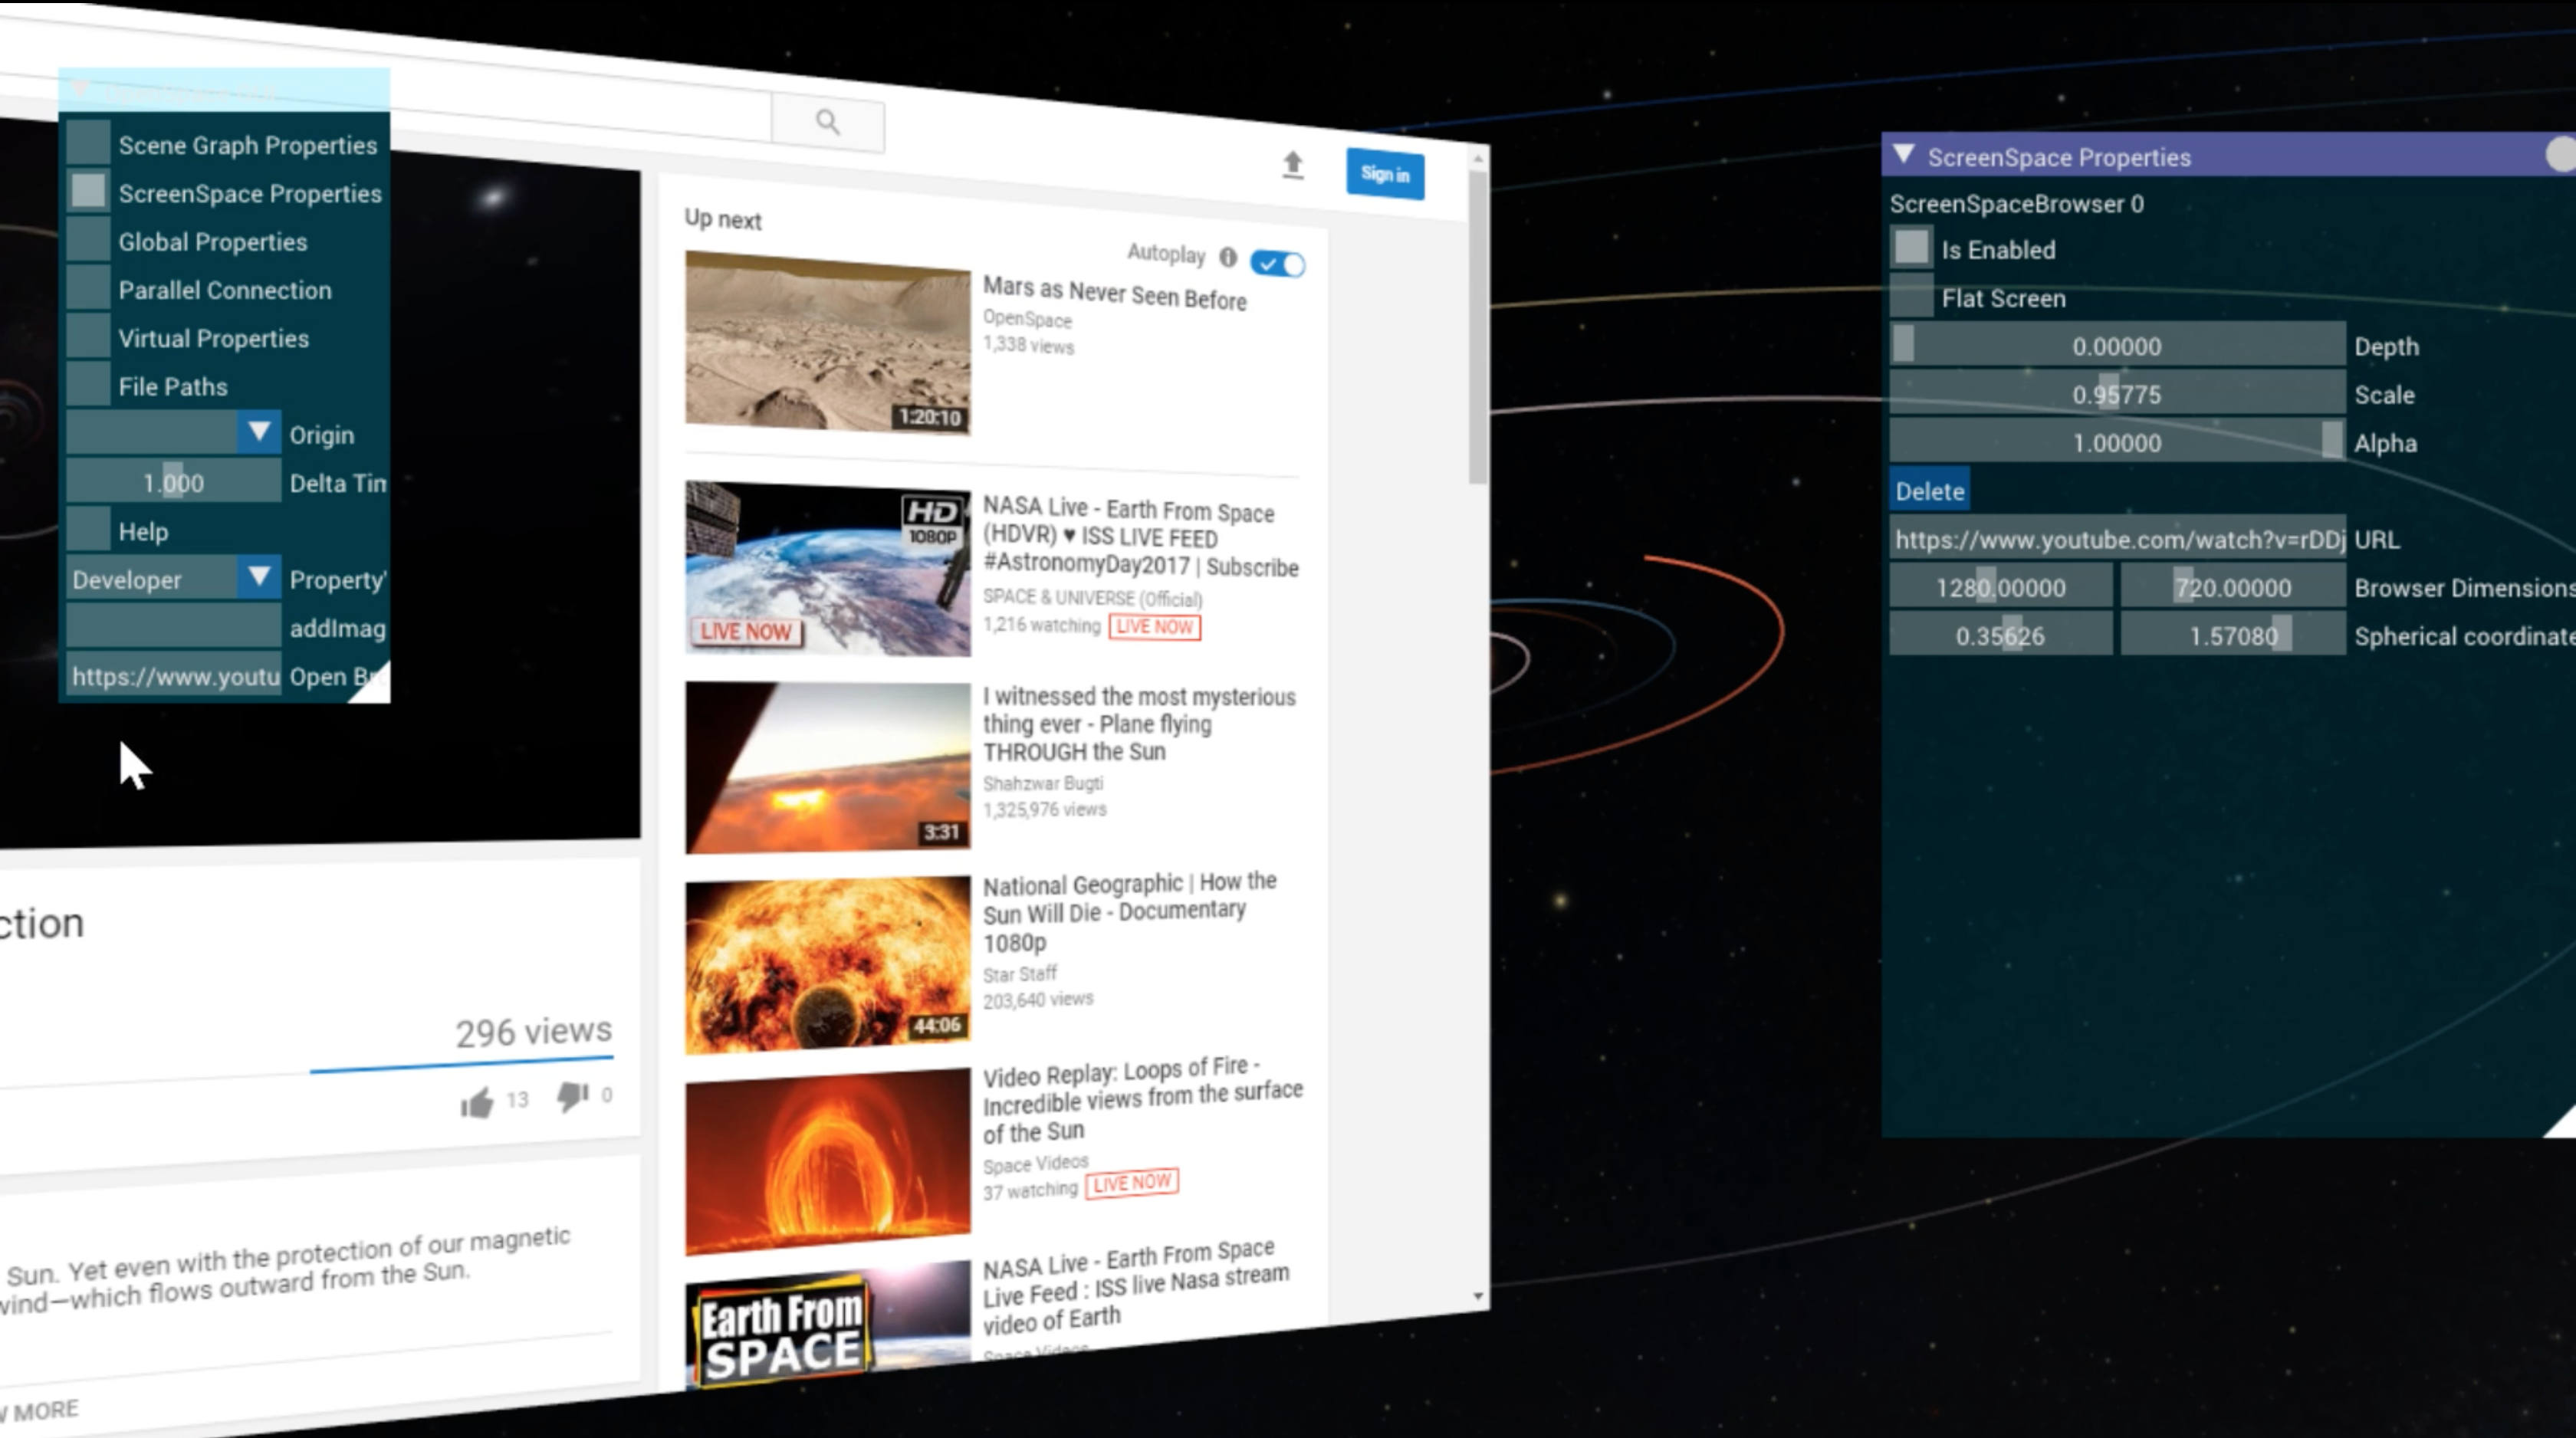
\includegraphics[width=0.7\linewidth]{./figures/screenspace.png}
\caption{\emph{The screen space browser with controls. The browser window is showing a video from the Openspace Youtube page.}}\label{fig:screenspace}
\end{figure}

The second is the screen-covering GUI browser. This is a transparent browser layer that covers the entire Openspace window. This is used to render the GUI on screen. See figure \ref{fig:guiprocess} for an early screen shot in the process of creating the GUI. While the screen space browser has a dynamic window size, allowing it to be changed as the user wants, the GUI browser's dimensions change as the window is resized.

\begin{figure}[!h]
\centering
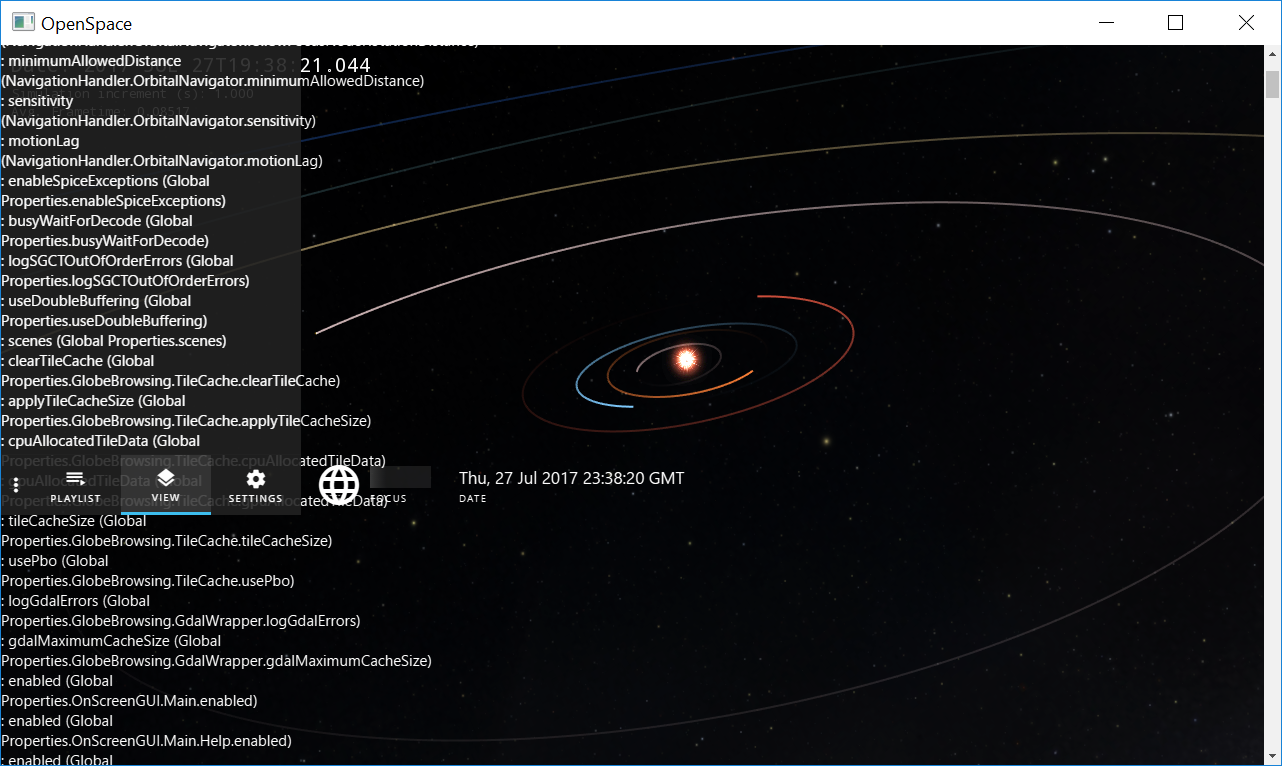
\includegraphics[width=0.7\linewidth]{./figures/guiprocess.png}
\caption{\emph{A screen shot from the GUI development, showing a misaligned sidebar and stringified JSON response from the simulation.}}\label{fig:guiprocess}
\end{figure}

\subsection{Event handling and interaction}\label{sec:interaction}

To handle events and interactions from the user, an event handler was created. This is a C++ class that holds a reference to a single active browser window within Openspace. This can be either a screen space window or the GUI window. This event handler listens to the events that gets captured by Openspace, which include keyboard button clicks, mouse movement, mouse button clicks and mouse scroll wheel movement. These get sent to the active browser windows using corresponding public methods.

To determine whether or not a mouse event should be captured, and blocked from triggering other parts of Openspace, a transparency layer mask is stored by each browser window. This is based on the assumption that an interaction over a transparent area won't trigger anything on the web page. See figure \ref{fig:maskweb} for an example view in the GUI and figure \ref{fig:maskmask} for its corresponding layer mask.

\begin{figure}[!h]
  \centering
  \subfloat[The GUI as it looks in Openspace, overlooking the surface of Mars.]{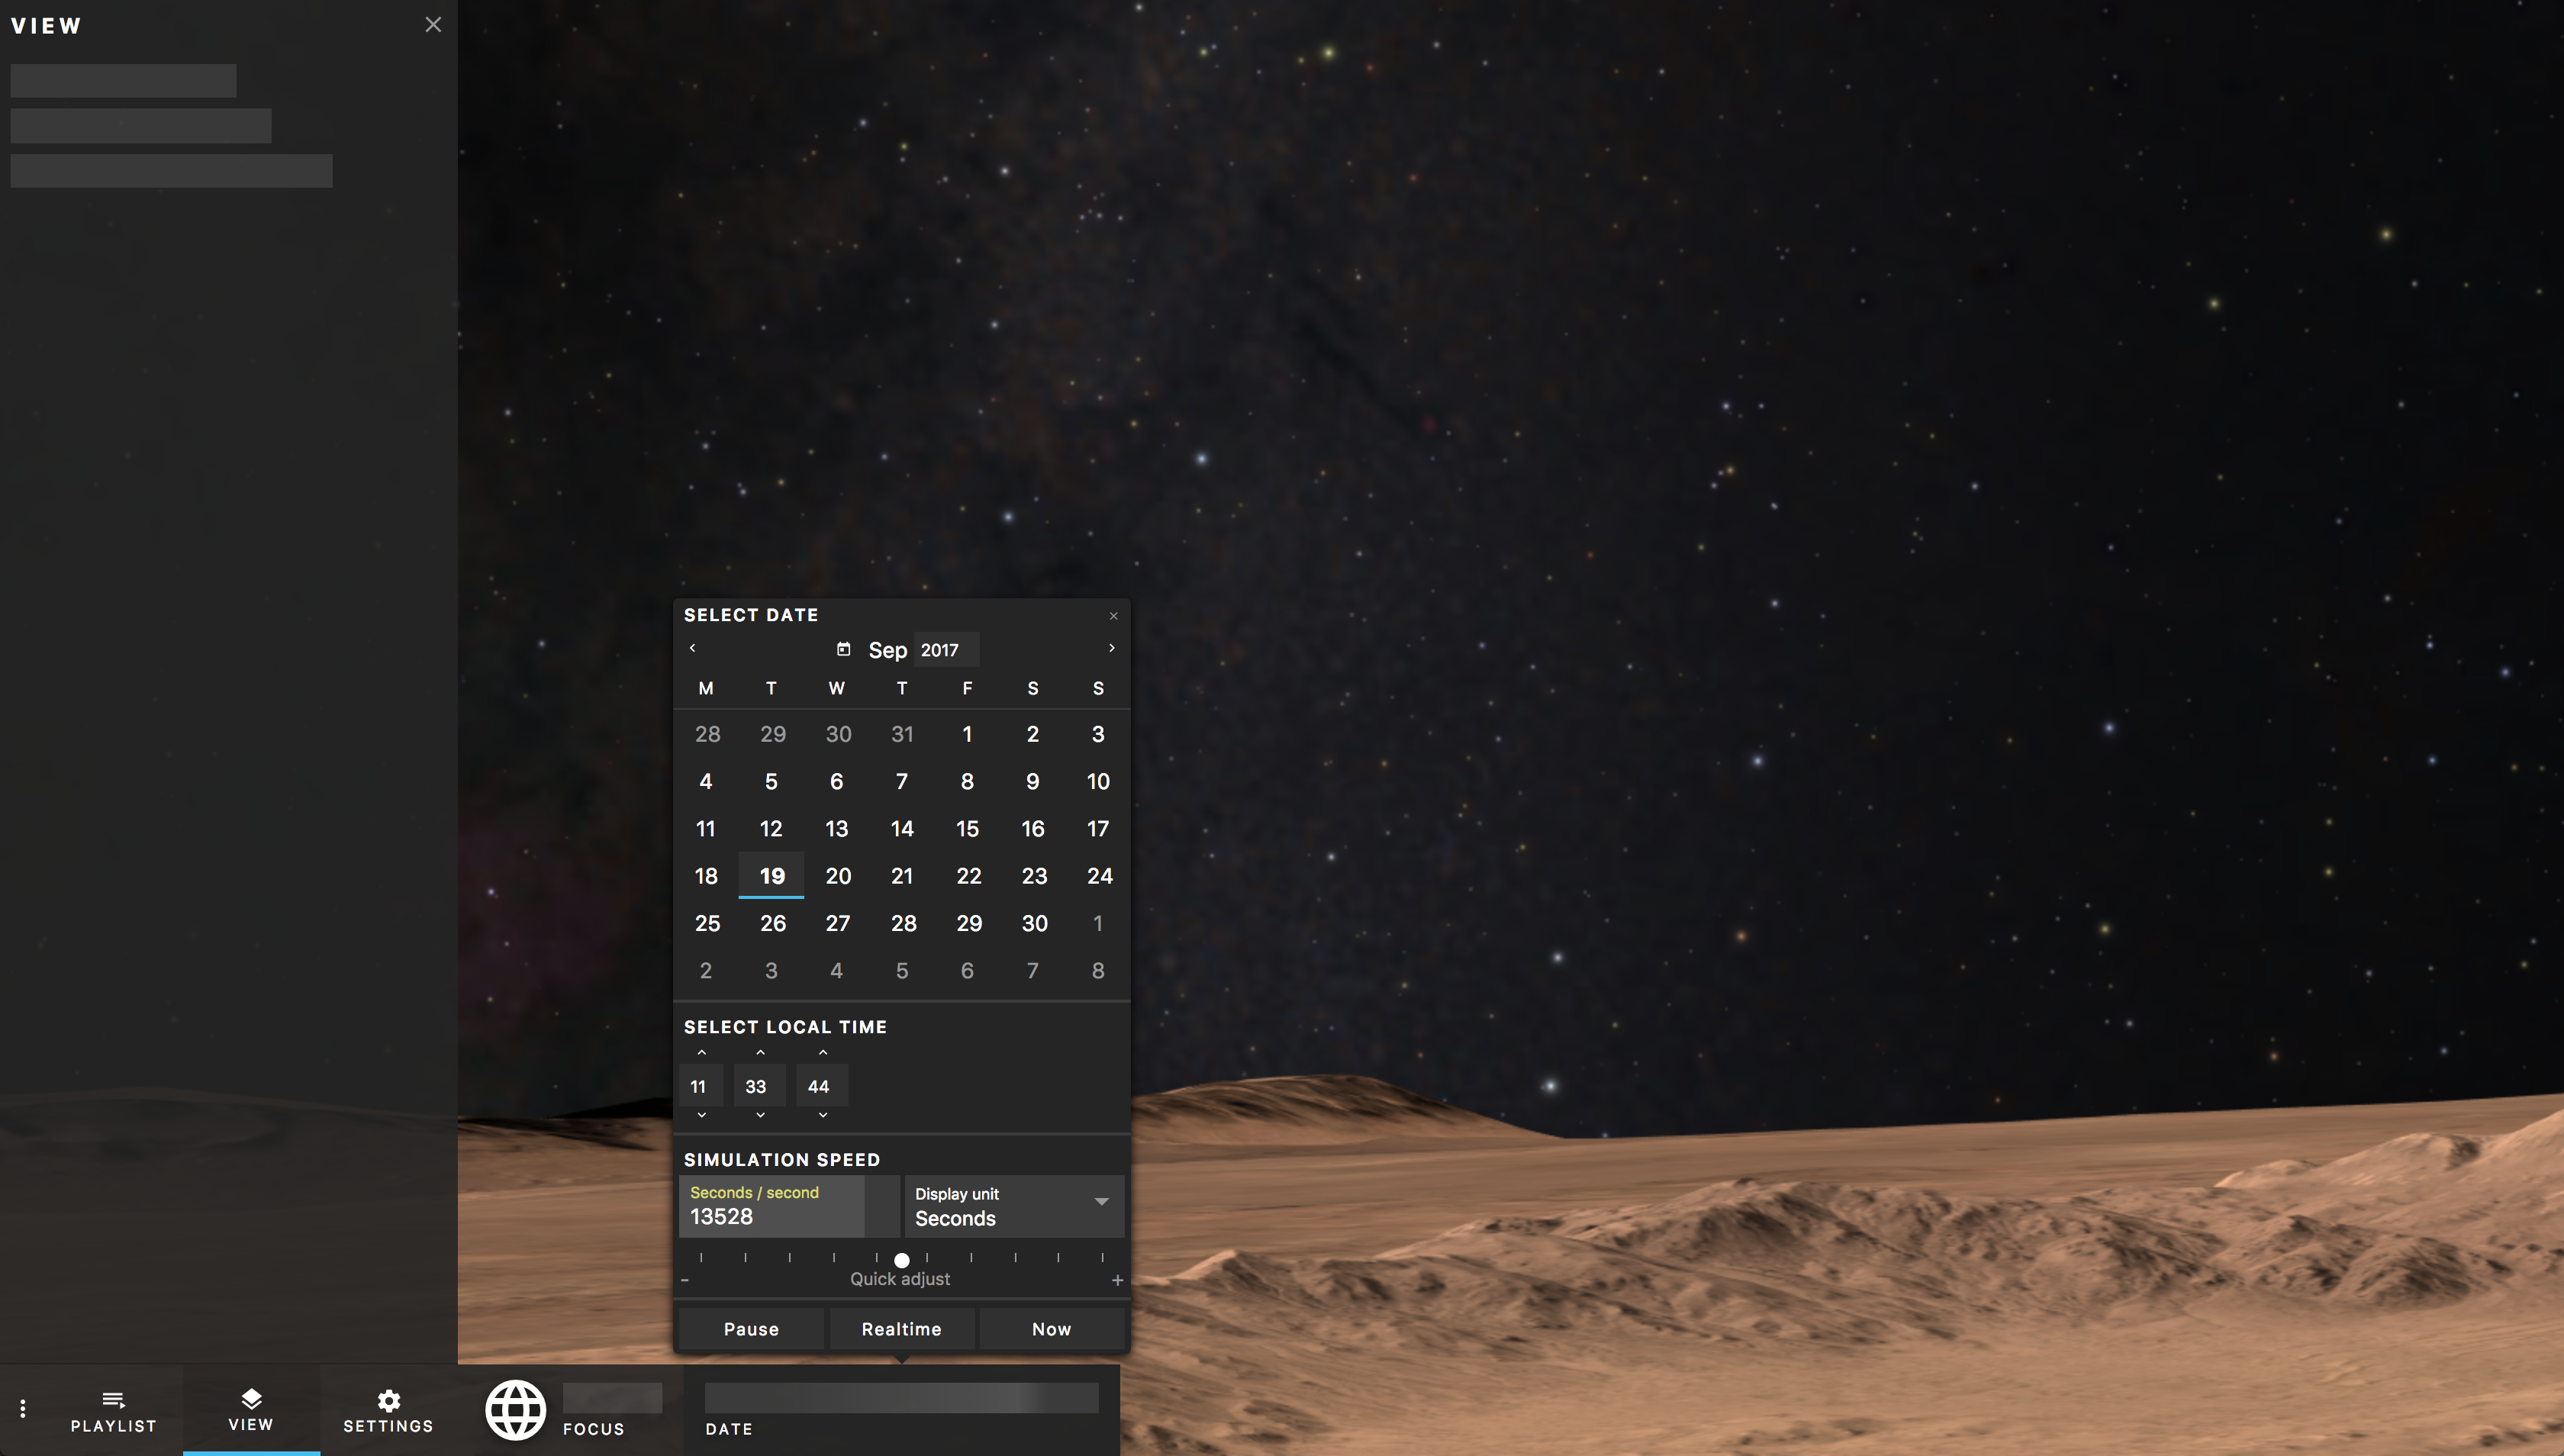
\includegraphics[width=0.45\textwidth]{./figures/maskweb.png}\label{fig:maskweb}}
  \hfill
  \subfloat[The layer mask. The black area will capture mouse clicks and mouse wheel movement.]{\fbox{
\includegraphics[width=0.45\textwidth]{./figures/maskmask.png}\label{fig:maskmask}}}
  \caption{The layer interaction mask}
\end{figure}

The layer mask is stored as a one-dimensional C++ array, and is updated every time the GUI is re-rendered. See more about the rendering in section \ref{sec:rendering}. When a user clicks inside the area marked as non-transparent, this will be sent to the GUI, and the event is captured. If the user clicks outside the area, the event will be ignored by the GUI, and the event trickles on within Openspace.

To get the index $i$ in the one-dimensional layer mask array from the coordinates $x$ and $y$, equation \ref{eq:coordtoidx} is used. Here, $W$ is the width of the browser window. This equation is used to decide whether or not the user's interaction is within an active area of the browser or not, as the position is given as coordinates in Openspace's event handlers.

\begin{equation}\label{eq:coordtoidx}
  i = x + y \cdot W
\end{equation}

\todo{figure with hit and miss on mask? is it needed?}

Keyboard button events, typing, is always sent to the GUI and never blocked. The phenomena caused by this, such as keyboard shortcuts getting unintentionally triggered, will later be discussed. \todo{discuss double effects of some key presses}

\begin{figure}[!h]
\centering
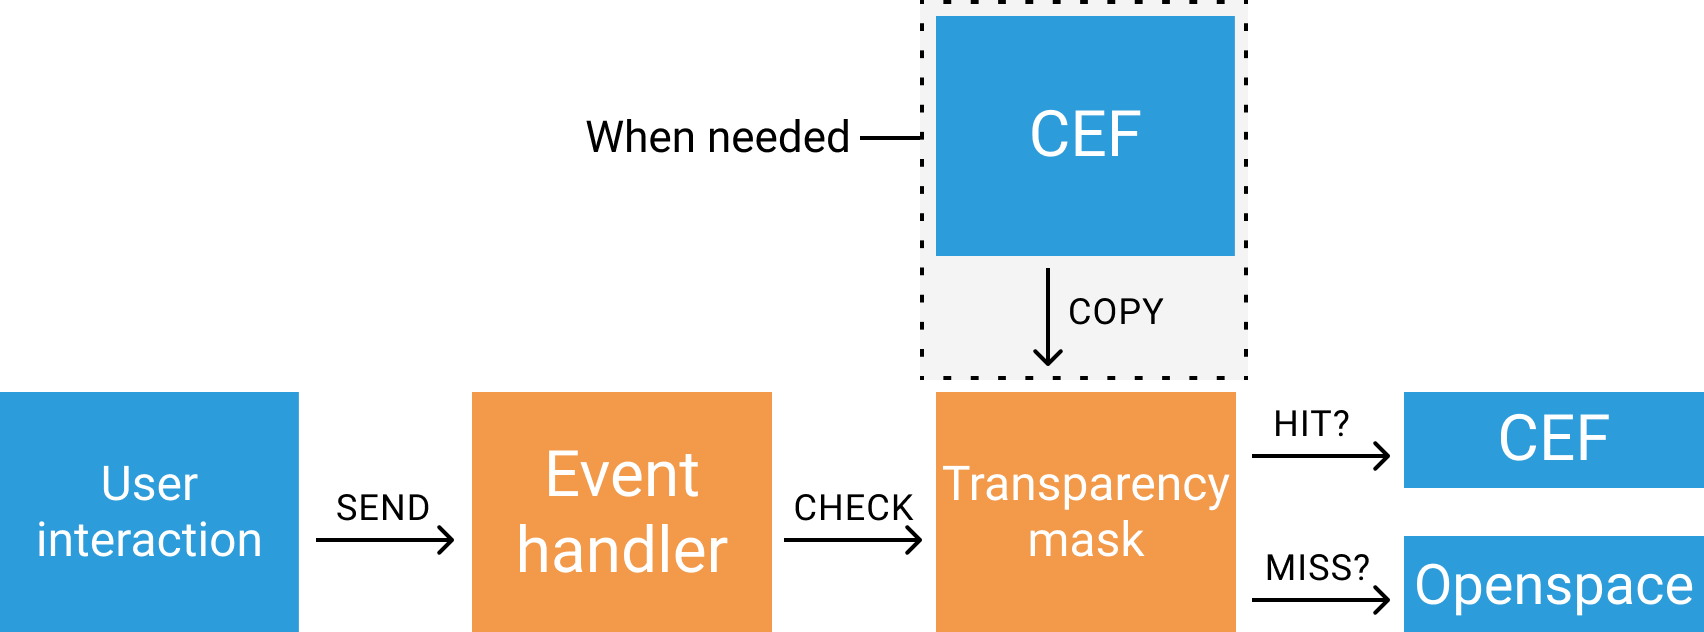
\includegraphics[width=0.9\linewidth]{./figures/maskupdate.png}
\caption{\emph{Overview of the mask update and user interaction process.}}\label{fig:maskupdate}
\end{figure}

When a browser window gets repainted, a buffer stored in the web renderer gets updated, see \ref{sec:rendering}. At this time, the layer mask also gets updated. To do this, the alpha channel of the RGBA values are extracted. If the alpha value of a pixel is non-zero, meaning that it is untransparent, this is considered a pixel that will capture the mouse events. See the life cycle of the interaction decision process in figure \ref{fig:maskupdate}.

\subsection{Rendering}\label{sec:rendering}

\begin{figure}[!h]
\centering
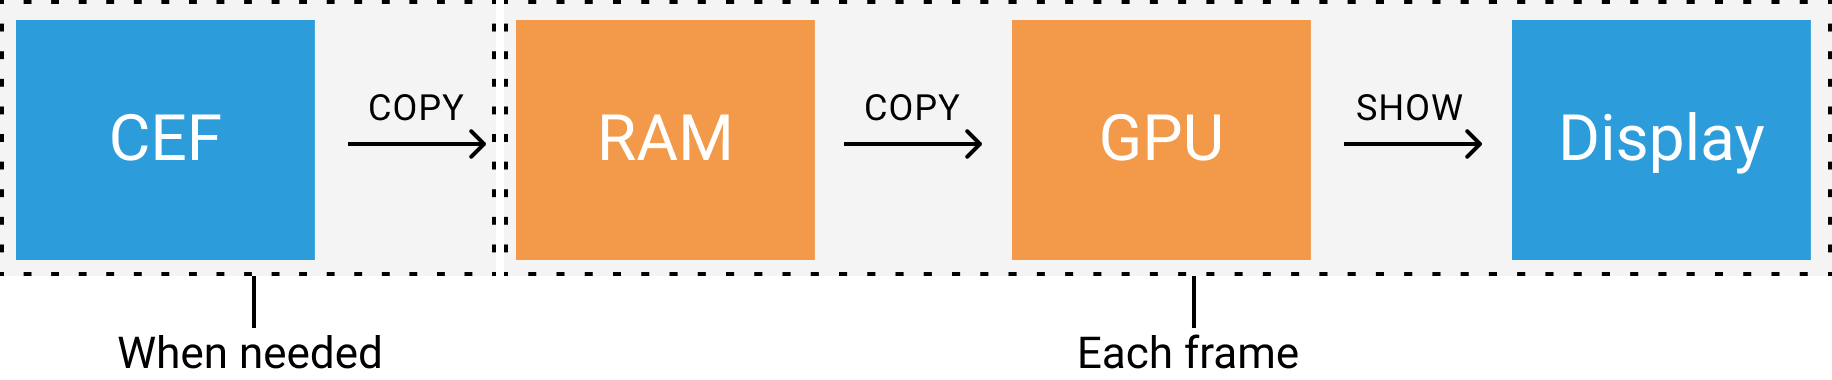
\includegraphics[width=0.9\linewidth]{./figures/rendering.png}
\caption{\emph{Overview of the rendering process.}}\label{fig:rendering}
\end{figure}

The rendering is a two-part process. First, CEF renders the web page to a buffer. This buffer is then copied on the working memory from CEF to the web browser implementation in Openspace. The buffer is then copied, each frame, to the GPU in the OpenGL pipeline in order to be drawn on the screen. The copying from CEF to Openspace is triggered only when the web page needs to be rendered, and the stored buffer is used until it gets updated and replaced by a new copy. See figure \ref{fig:rendering} for an overview of the steps in the rendering process.

To reduce the computing power needed, CEF only updates the buffer when something on the web page gets changed and a repaint of the web page is needed. This can be a colour changing, text changing, box moving or anything similar. Regardless of the magnitude of the change or the cause of this change, the whole buffer gets replaced. This affects both the transparency mask mentioned in section \ref{sec:interaction} and the buffer that gets copied to the GPU for rendering. Depending on the internal bandwidth of the computer, this copying from the RAM to the GPU might be a time consuming task, affecting the performance of the simulation. The implications of this will be discussed later. \todo{discuss ram to gpu copying}

\section{Socket server and simulation control}
\section{GUI development}
